\section{Anhang}\label{sec:anhang} % (fold)
\begin{listing}[htbp]
\begin{minted}[xleftmargin=20pt,linenos,breaklines,fontsize=\scriptsize]{js}
const rawData = $json["content"];
const lines = rawData.split('\n');
const formFields = [];

lines.forEach((line, index) => {
  const cleanedLine = line.replace(/^\d+\.\s*/, '');
  const braceMatches = [...cleanedLine.matchAll(/\{([^}]+)\}/g)];
  let rawValues = [];

  if (braceMatches.length > 0) {
    braceMatches.forEach(m => {
      rawValues.push(...m[1].split(',').map(v => v.trim()));
    });
  } else {
    rawValues = cleanedLine.split(',').map(v => v.trim());
  }

  if (rawValues.length < 3) return;

  const [name, max_amount_raw, current_amount_raw] = rawValues;
  const max_amount = parseInt(max_amount_raw, 10);
  const current_amount = parseInt(current_amount_raw, 10);

  if (isNaN(max_amount) || isNaN(current_amount)) return;

  formFields.push({
    fieldLabel: `name: ${name}, max amount: ${max_amount}, current amount: ${current_amount}`,
    placeholder: 'enter if you want it changed',
    requiredField: false
  });
});

return formFields.map(field => ({ json: field }));
\end{minted}
\caption{JavaScript Code zur Aufbereitung der Daten für die Validierung}
\label{lst:descr:js:code1}
\end{listing}

\begin{listing}[htbp]
\begin{minted}[xleftmargin=20pt,linenos,breaklines,fontsize=\scriptsize]{js}
// Loop over input items and add a new field called 'myNewField' to the JSON of each one
let out = { preferenzen: $('Edit Fields').first().json.preferenzen, personen: $('Edit Fields').first().json.personen, products: [] }
for (const item of $input.all()) {
  for (const element in item.json) {
    if (element == "submittedAt" || element == "formMode") {
      delete item.json[element]
      continue
    }
    const placeholder = element
    const product = item.json[element] || placeholder
    if (!product) {
      continue
    }
    out.products.push(product)
  }
}
return out;
\end{minted}
\caption{JavaScript Code zur Nachbereitung der Daten nach der Validierung}
\label{lst:descr:js:code2}
\end{listing}

\begin{listing}[htbp]
\begin{minted}[xleftmargin=20pt,linenos,breaklines,fontsize=\scriptsize]{json}
{
  "type": "object",
  "properties": {
    "Cocktails": {
      "type": "array",
      "items": {
        "type": "object",
        "required": [
          "Name",
          "Zutaten",
          "Beschreibung",
          "fehlende Zutaten"
        ],
        "properties": {
          "Name": {
            "type": "string"
          },
          "Beschreibung": {
            "type": "string"
          },
          "Zutaten": {
            "type": "array",
            "items": {
              "type": "object",
              "required": [
                "Zutat",
                "Menge"
              ],
              "properties": {
                "Zutat": {
                  "type": "string"
                },
                "Menge": {
                  "type": "string"
                }
              }
            }
          },
          "fehlende Zutaten": {
            "type": "array",
            "items": {
              "type": "string"
            }
          }
        }
      }
    }
  }
}
\end{minted}
\caption{KI-Modell Antwort-Format der Rezeptvorschläge}
\label{lst:descr:js:code3}
\end{listing}

\begin{listing}[htbp]
\begin{minted}[xleftmargin=20pt,linenos,breaklines,fontsize=\scriptsize]{js}
const BASE = $env["SHOPPING_URL"] ?? "http://localhost:3069";

const cocktails = $input.all().map(all => all.json);

const htmlEntries = cocktails.map( (cocktail) => {
  const zutatenArr = cocktail.Zutaten || [];
  const fehlendeArr = cocktail['fehlende Zutaten'] || [];

  const zutaten = zutatenArr.map(z => `${z.Menge} ${z.Zutat}`).join(', ');
  const fehlende = fehlendeArr.join(', ');
  const bucketId = cocktail.uuid;

  let linkBlock = '';

  const link = `${BASE}/?shopping=${bucketId}`;
    linkBlock = `
      <p>
        <a href="${link}" target="_blank" rel="noopener">Zur Einkaufsliste</a><br>
        <small>Liste-ID: ${bucketId}</small>
      </p>
    `;

  return `
    <div class="entry">
      <h3>${cocktail.Name}</h3>
      <p>${cocktail.Beschreibung}</p>
      <h4>Zutaten:</h4>
      <p>${zutaten}</p>
      <h4>Fehlende Zutaten:</h4>
      <p>${fehlende || '-'}</p>
      ${linkBlock}
    </div>
  `;
});

return { html: htmlEntries.join('\n') };
\end{minted}
\caption{JavaScript Code zur Vorbereitung der Ergebnisdarstellung}
\label{lst:descr:js:code4}
\end{listing}

\begin{listing}[htbp]
\begin{minted}[xleftmargin=20pt,linenos,breaklines,fontsize=\scriptsize]{css}
body {
  font-family: 'Open Sans', sans-serif;
  background-color: #f0f0f0;
  margin: 0;
  padding: 2rem;
}
h1 {
  margin-bottom: 2rem;
}
.header div {
  background: white;
  border-radius: 0.5rem;
  box-shadow: 0 2px 6px rgba(0,0,0,0.1);
  padding: 1rem;
  max-width: 500px;
  margin: 1rem auto 1rem auto;
}

div h4 {
  margin-top: 1rem;
}
\end{minted}
\caption{CSS Code um dem Auge beim Erblicken des Ergebnisses zu schmeicheln}
\label{lst:descr:js:code5}
\end{listing}
\clearpage
\begin{figure}
    \begin{center}
        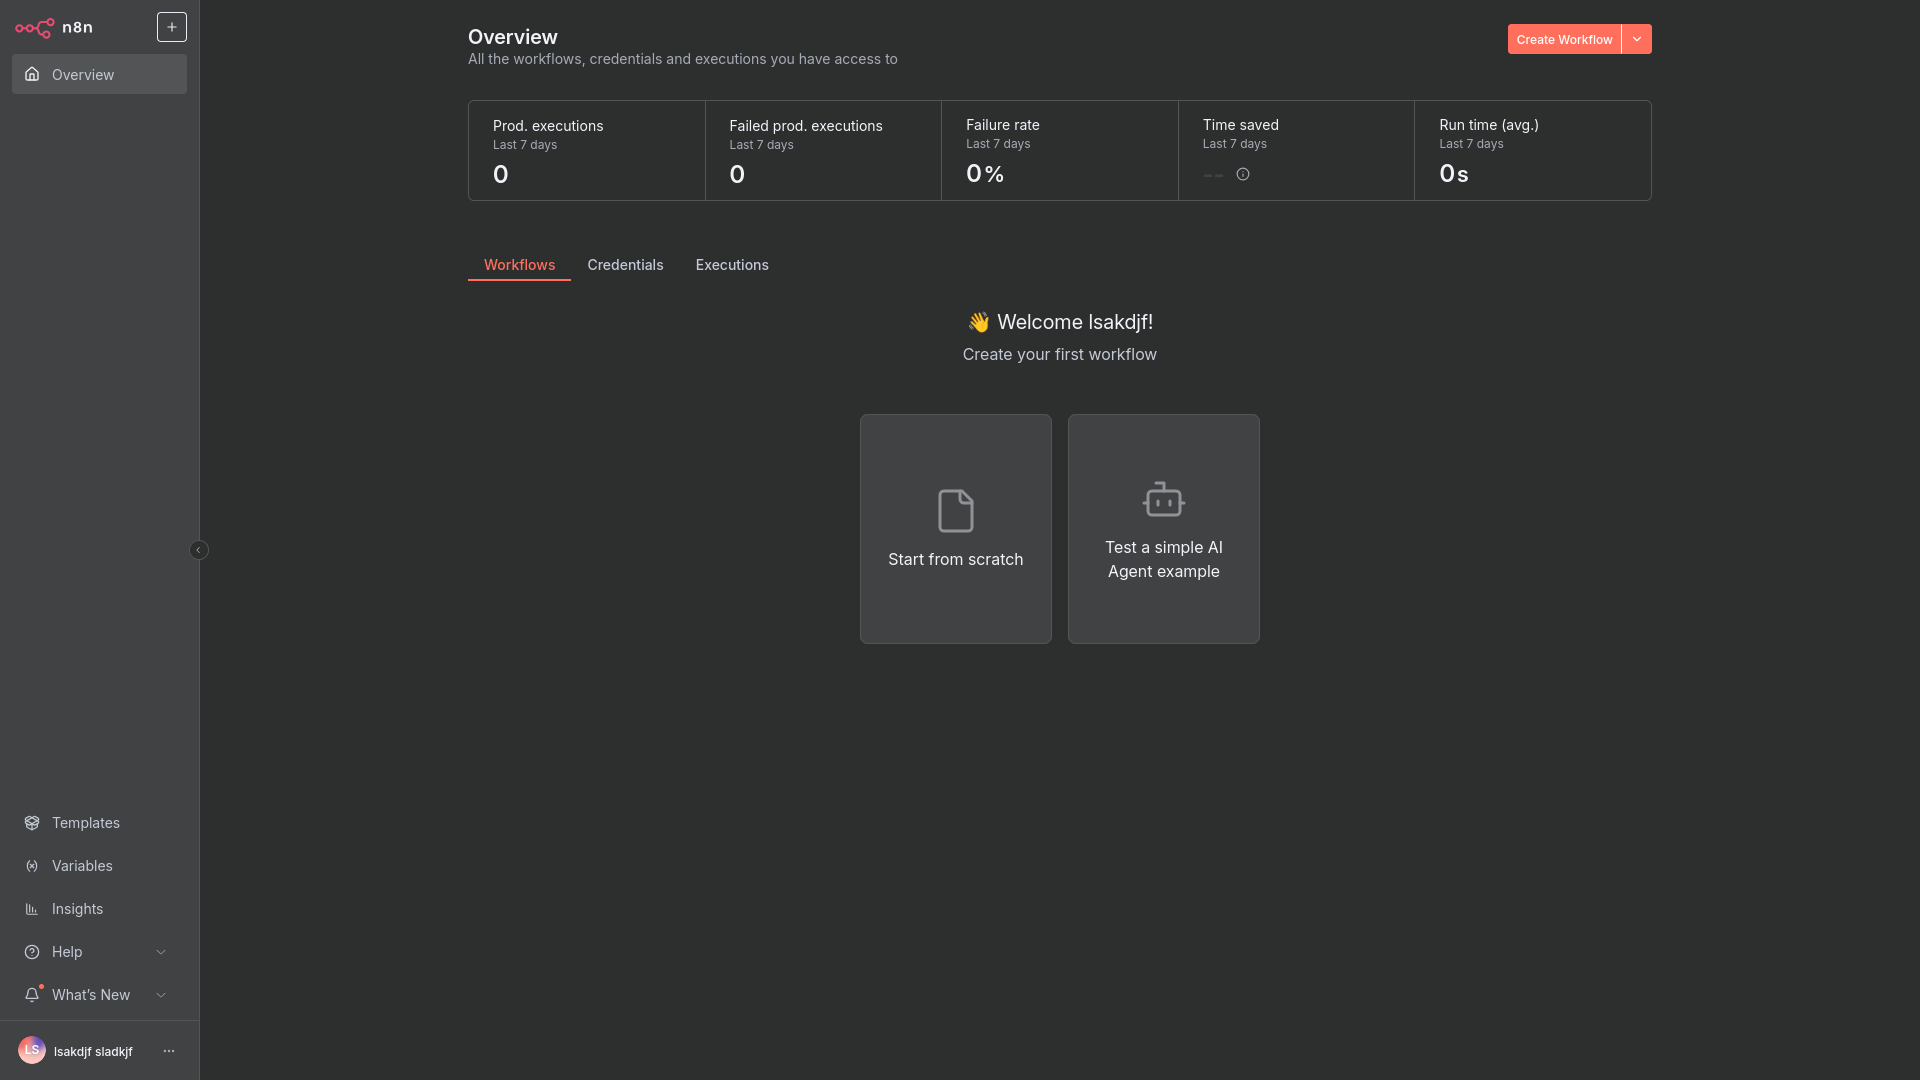
\includegraphics[width=0.95\textwidth]{images/n8n_overview.png}
    \end{center}
    \caption{n8n Übersichtsseite}\label{fig:n8n_overview}
\end{figure}

\begin{figure}
    \begin{center}
        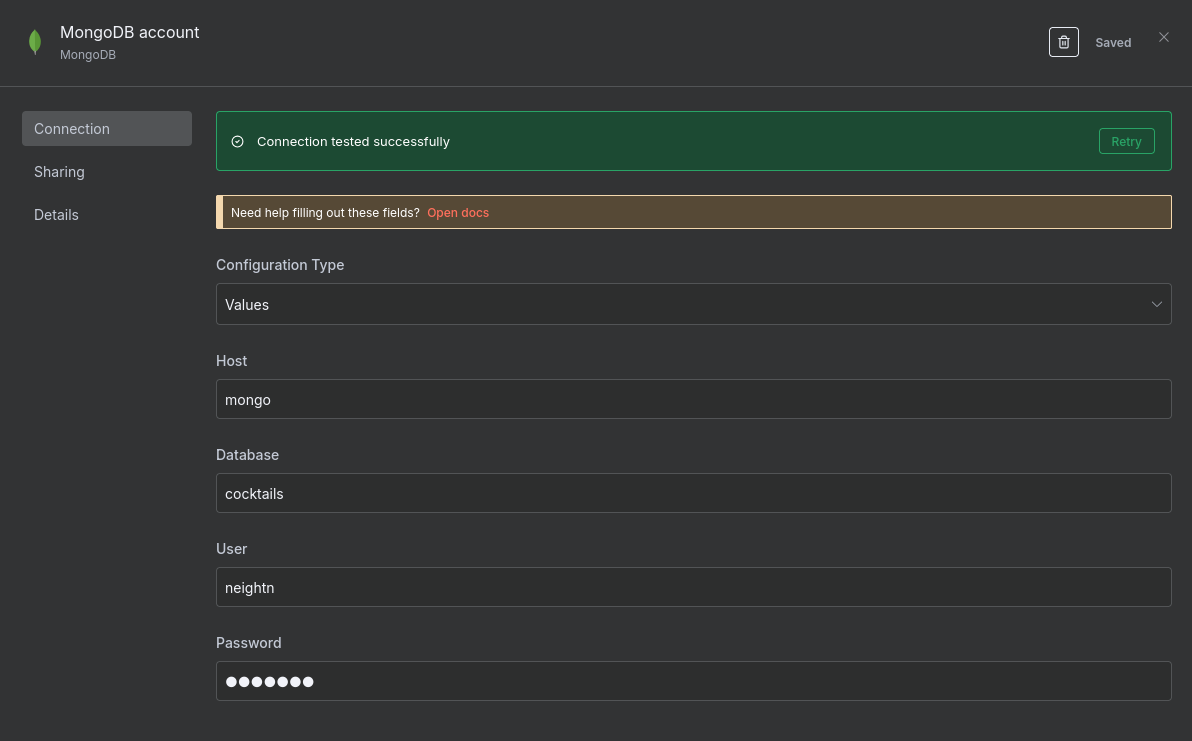
\includegraphics[width=0.95\textwidth]{images/n8n_mongo_creds.png}
    \end{center}
    \caption{n8n MongoDB Zugangsdaten}\label{fig:n8n_mongo_creds}
\end{figure}

\begin{figure}
    \begin{center}
        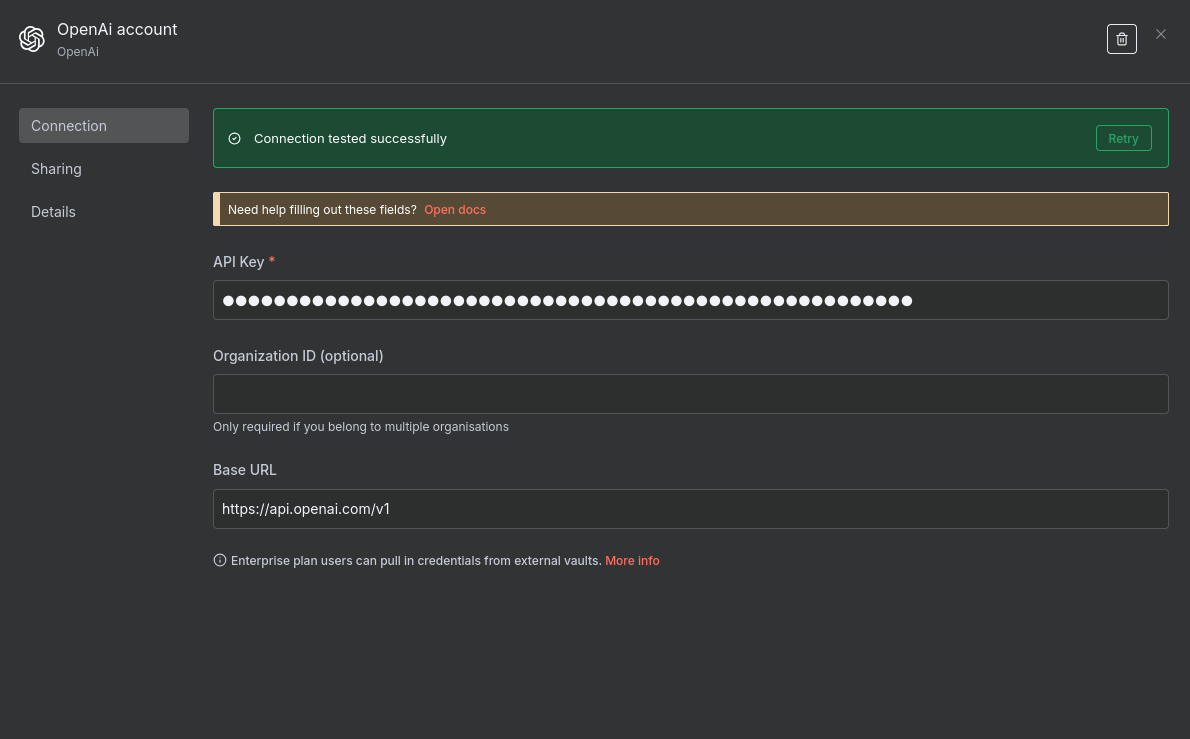
\includegraphics[width=0.95\textwidth]{images/n8n_openai_creds.png}
    \end{center}
    \caption{n8n OpenAI Zugangsdaten}\label{fig:n8n_openai_creds}
\end{figure}

\begin{figure}
    \begin{center}
        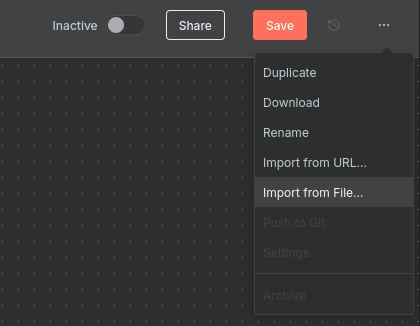
\includegraphics[width=0.95\textwidth]{images/n8n_import.png}
    \end{center}
    \caption{n8n Import Workflow}\label{fig:n8n_import}
\end{figure}
